\qns{Transistor Switch Model}
\qcontributor{Ryan Koh}
\qcontributor{Son Tran}

You have two CMOS inverters made from NMOS and PMOS devices. Both NMOS and PMOS devices
have an "on resistance" of $R_{on}=\SI{1}{\kilo\ohm}$, and each has a gate capacitance (input capacitance) of $C=\SI{1}{\femto\farad}$
(femto-Farads = $10^{−15}$). We assume the "off resistance" (the resistance when the transistor is off) is infinite
(i.e., the transistor acts as an open circuit when off). The supply voltage VDD is $\SI{1}{\volt}$. The two inverters are
connected in series, with the output of the first inverter driving the input of the second inverter.
\begin{figure} [h!]
	\centering
	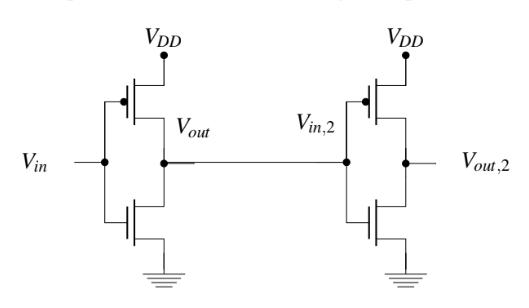
\includegraphics{\bank/ode/figures/transwitchmodel_cmos.png}
	\caption{CMOS Inverter}
	\label{fig:cmos}
\end{figure}

Consider the circuit below, assume that when $t\leq0$, the capacitor has no charge stored $(V_{\text{c}}(t=0) = 0)$. At $t=0$, the switch closes. Assume that $V_s=\SI{5}{\volt}$, $R=\SI{100}{\ohm}$, and $C=\SI{10}{\micro\farad}$. 

\begin{figure}[H]
	\begin{centering}
		\begin{circuitikz}
			\draw (0, 4)
			to[V =$V_s$] (0, 0);
			\draw (0, 4)
			to[switch,l^=\mbox{$t = 0$}](4,4)
			(4,4) to[R = $R$,v=$V_R(t)$,i>^=$i_R(t)$] (7,4)	
			to [short] (9,4)
			to[C = $C$, v=$V_C(t)$,i>^=$i_C(t)$] (9,0)
			to [short] (0,0);
		\end{circuitikz}
		\caption{\label{fig:circuit}RC Circuit with Voltage Source}
	\end{centering}
\end{figure}


\begin{enumerate}

\qitem Assume the input to the first inverter has been low ($V_{in} = \SI{0}{\volt}$) for a long time, and then switches
at time $t = 0$ to high ($V_{in} = V_{DD}$). \textbf{Draw a simple RC circuit and write a differential equation describing the output voltage of the first inverter for time $t \geq 0$.} Don’t forget that the second inverter is “loading” the output of the first inverter — you need to think about both of them.

\sol {
\begin{align*}
\intertext{The input to the first inverter was low for a long time. This means the output of the
inverter had been held at high for a long time. To analyze this circuit as an RC circuit we can recall
the transistor switch model. Using this we can see that the first inverter’s output appears as a resistor
connected to $V_{DD}$ when the input is low or a resistor connected to ground when the input turns high.} \\ \\
\intertext{The second inverter "loads" the output of the first inverter. Modeling the
gates of the transistors as capacitors, these gates together form our capacitive load. The gate of the
PMOS acts as a capacitor to $V_{DD}$ and the gate of the NMOS acts as a capacitor to ground.} \\ \\
\intertext{We can then draw the following RC circuit:}
\begin{figure} [h!]
	\centering
	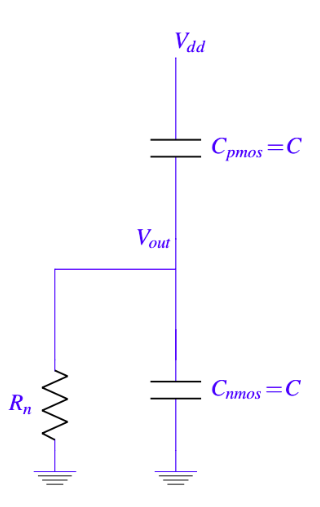
\includegraphics{\bank/ode/figures/transwitchmodel_first_inverter.png}
	\caption{Inverter Output at 0}
	\label{fig:inverter0}
\end{figure}
\intertext{To get the differential equation describing the output of the first inverter at time $t \geq 0$ let us first think about the behavior of the circuit at and after $t = 0$.} \\
\intertext{At $t = 0$ we know that the output $V_{out} = V_{DD}$. This means that $C_{nmos}$ is charged while the $C_{pmos}$ is not as there is no voltage difference across it. When the input to the inverter changes the output goes to zero in steady state.} \\ \\
\intertext{For this to occur the $C_{pmos}$ must start discharging and $C_{nmos}$ must start charging to $V_{DD}$. We know the
voltage across $C_{pmos}$ is $V_{out}(t) - V_{DD}$ and the voltage across $C_{nmos}$ is $V_{out}(t)$. Using this information we can set up a differential equation to solve for $V_{out}(t)$:}
I_{c_{pmos}} = C_{pmos} \frac{d}{dt}(V_{out}(t) - V_{DD}) \\
I_{c_{nmos}} = C_{nmos} \frac{d}{dt}V_{out}(t) \\
I_{R_{on}} = \frac{V_{out}(t)}{R_{on}} \\
I_{c_{pmos}} + I_{c_{nmos}} = -I_{R_{on}} \\
C_{pmos} \frac {d}{dt} (V_{out}(t) - V_{DD}) + C_{nmos} \frac {d}{dt} V_{out}(t) = - \frac {V_{out}(t)}{R_{on}} \\
C_{pmos} \frac {d}{dt} V_{out}(t) + C_{nmos} \frac{d}{dt} V_{out}(t) = - \frac {V_{out} (t)} {R_{on}} \\
(C_{pmos} + C_{nmos}) \frac {d}{dt} V_{out} (t) = - \frac {V_{out}(t)} {R_{on}} \\
\frac {d}{dt} V_{out}(t) = - \frac {V_{out} (t)} {R_{on} (C_{pmos} + C_{nmos})} \\
\frac {d}{dt} V_{out} (t) = - \frac {V_{out} (t)} {R_{on} (2C)}
\end{align*}
}

\qitem Write out the KCL equations associated with the circuit when the switch is open. Then write out the differential equations for the case when the switch is closed.

\meta{
	Testing meta here
}

\sol{
\begin{align*}
\intertext{When the swtich is open, we denote the voltage to the left of resistor to be $y$. We obtain the following differential equations. KCL at node between the resistor and capacitor gives}
\frac{y - V_{\text{C}}}{R} = C\frac{dV_{\text{C}}}{dt} \\
\intertext{Since the current going into the resistor and the voltage source is zero, KCL gives:}
\frac{y - V_{\text{C}}}{R} = 0 \\
\intertext{and}
i_{\text{Vs}} = 0\\
\intertext{When the switch is closed, the following still holds:}
\frac{y - V_{\text{C}}}{R} = C\frac{dV_{\text{C}}}{dt} \\
\intertext{Additionally, KCL at the node between the resistor and voltage sources gives:}
\frac{V_{\text{S}} - V_{\text{C}}}{R} +  i_{\text{Vs}} = 0
\end{align*}
}



\qitem Write out the differential equation for $V_{\text{c}}(t)$ after the switch closes.

\sol{
\begin{align*}
\intertext{From the previous problem we know that when the switch is closed,}
\frac{V_{\text{S}}- V_{\text{C}}}{R} = C\frac{dV_{\text{C}}}{dt} \\
\intertext{Thus we obtain}
C\frac{dV_{\text{C}}}{dt} + \frac{V_{\text{C}}}{R} - \frac{V_{\text{S}}}{R}=0
\end{align*}
}



\qitem What is the initial condition for $V_{\text{c}}(t)$ (i.e. $V_{\text{c}}(t=0)$) and what is $V_{\text{c}}(t \to \infty)$?

\sol{

\begin{align*}
\intertext{No charge is on the capacitor before time $t=0$. Using $q=VC$, we know that $V_{\text{c}}=\SI{0}{\volt}$ before $t=0$.}
\intertext{At $t=0$, the switch closes. Since voltage across the capacitor cannot change instantaneously,}
V_{\text{c}}(t=0)&=0. \\
\intertext{As $t$ goes to infinity, the capacitor will become fully charged and the current goes to zero. Therefore, the voltage of the capacitor equals the voltage source:}
V_{\text{c}}(t \to \infty)&=V_{\text{S}}.
\end{align*}
}




\qitem Using the initial conditions found in the previous parts, find an expression for $V_{\text{c}}(t)$ in terms of $V_{\text{s}}$, $R$, and $C$.

\sol{
	\begin{align*}
		\intertext{The general solution to the equation}
		\frac{dy}{dt}&=\lambda y \\
		\intertext{is}
		y(t)&=Ke^{\lambda t}, \\
		\intertext{where $K$ is a constant and $\lambda$ is the eigenvalue of the equation. In our case, we know}
		C\frac{dV_{\text{C}}}{dt} + \frac{V_{\text{C}}}{R} - \frac{V_{\text{S}}}{R}=0,\\
		\intertext{which can be written as}
		\frac{dV_{\text{C}}}{dt} = - \frac{V_{\text{C}}}{RC} + \frac{V_{\text{S}}}{RC}.\\
		\intertext{The solution will be in the form}
		V_{\text{c}}(t)&=Ke^{-\frac{t}{RC}} + V_{\text{S}}. \\
		\intertext{To find $K$, we can plug in our initial condition at $t=0$:}
		V_{\text{c}}(t=0)&=K + V_{\text{S}} = 0.\\
		\intertext{So our overall equation ends up being}
		V_{\text{c}}(t)&=-V_{\text{S}} e^{-\frac{t}{RC}} + V_{\text{S}}. \\
		% % I_{\text{c}}(t=0)&=Ke^{-\frac{0}{RC}}=\frac{V_{\text{s}}}{R} \\
		% % \intertext{From this we can see}
		% % K&=\frac{V_{\text{s}}}{R} \\
		% % \intertext{So our overall equation ends up being}
		% % I_{\text{c}}(t)&=\frac{V_{\text{s}}}{R}e^{-\frac{t}{RC}} \\
		\intertext{We can also double check our answer by looking at the state for t $\to \infty$:}
		V_{\text{c}}(t \to \infty)&=-V_{\text{S}} e^{-\infty} + V_{\text{S}} =  V_{\text{S}},\\
		\intertext{which agrees with our answer from previous part.}
	\end{align*}
}

\qitem On what order of magnitude of time (nanoseconds, milliseconds, 10's of seconds, etc.) does this circuit settle ($V_{\text{c}}$ is $>95\%$ of its value as $t \to \infty$)?

\sol{

\begin{align*}
\intertext{The time constant $\tau$ of an RC circuit is just $\tau = RC$. For our circuit:}
\tau &= RC = \SI{100}{\ohm} \cdot \SI{10}{\micro\farad} = \SI{0.001}{\second} \\
\intertext{After 3 time constants, the voltage will be ~95\% of its steady state value}
3\tau &= \SI{0.003}{\second} \\
\intertext{The circuit will settle on the order of milliseconds.}
\end{align*}

}

\qitem Give 2 ways to reduce the settling time of the circuit if we are allowed to change one component in the circuit.

\sol{

To reduce settling time, reduce $\tau$. We can achieve this by

\begin{enumerate}
\item Lowering the value of $R$ or
\item Lowering the value of $C$.
\end{enumerate}

Notice how the value of $V_{\text{s}}$ does not change the settling time.

}


\end{enumerate}
